\section{Problemas de valores de contorno (PVC)}
Para este tipo de ejercicios también, es \textbf{siempre hacer lo mismo}. Te aprendes a como armar la matriz y las 2 formulas (tal vez 3) de diferenciación y después es todo mecánico. Vas a ver que te van a pedir utilizar metodos vistos en clase para resolver sistemas de ecuaciones. Anda a la fácil, usa Gauss-Seidel o Jacobi (ahre que son las unicas. Porque SOR no vas a usarlo, querete un poco).


\subsection{6/08/24}

Sea la ecuación diferencial

$$\frac{d^2y}{dx^2} + \frac{y}{4} = 0$$

con $y_0 = 1$ y $y_\pi = 0$

Plantear su resolución numerica usando diferencias finitas centradas. Expresar el sistema de ecuaciones resultantes en forma matricial. Considerar que el dominio se divide en $N + 1$ tramos.

\begin{enumerate}
    \item[a)] Obtener la solución aproximada para $N = 1$ (1 punto)
    \item[b)] Repetir para $N = 3$. Usar métodos vistos en el curso para resolver sistema lineal(2 puntos)
    \item[c)]Estimar el valor de $y(\frac{\pi}{2})$(1 punto)
\end{enumerate}

\subsubsection{Punto a}

Que nos digan que el dominio esta dividido en $N + 1$ tramos nos dice que va a haber $N$ puntos sin contar los bordes.


Discretizamos. Para esto utilizamos las formulas de las preliminares. 


$$
y''(x_i) = \frac{y(x_{i+1}) - 2y(x_i) + y(x_{i-1}) }{h^2}
$$

Ahora lo que hacemos es reemplazamos en la ecuación diferencial original. 



$$
\frac{y(x_{i+1}) - 2y(x_i) + y(x_{i-1}) }{h^2} + \frac{y_n}{4} = 0
$$


Multiplicamos $h^2$ en ambos miembros, agrupamos y reorganizamos. 


$$
    \textcolor{green}{(1)}y_{n+1} + \textcolor{blue}{(-2 + \frac{h^2}{4})}y_n + \textcolor{red}{(1)}y_{n-1} = 0  
$$

Bien, acá remarcamos los coeficientes que multiplican a las $y$ porque son los que van a ir a las matrices. 

Así que con esto, podemos armar la matriz generica. Recordemos como queda la parte después del igual de la matriz: 
\newpage
\begin{figure}[h!]
    \centering
    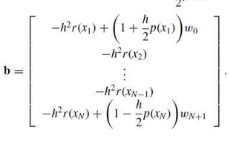
\includegraphics[width=0.5\linewidth]{b_matrix_pvc.png}
    \caption{Sistema tridiagonal}
    \label{fig:enter-label}
\end{figure}

Como podes observar, en el primer elemento esta el $-h^2 r(x_1)$, Que es lo que queda a la derecha del igual de la ecuación diferencial ya despejada y ya discretizada. Y después tiene un $(\dots)w_0$, ese $w_0$ es el dato que te dan de $y_0$. Para la primera iteración pasas el $y_{n-1}$ para el otro lado del igual, y el valor que lo acompaña es su coeficiente. La matriz es \textbf{siempre igual}.

Sabiendo esto, vamos a armar la matriz: 

\[
\begin{bmatrix}
\textcolor{blue}{(-2 + \frac{h^2}{4})} & \textcolor{green}{(1)} & 0 & \dots & 0 \\
\textcolor{red}{(1)} & \textcolor{blue}{(-2 + \frac{h^2}{4})} & \textcolor{green}{(1)} & \dots & 0 \\
\dots  & \dots  & \dots  & \dots & \dots  \\
0 & 0 & \dots & \textcolor{green}{(1)} & \textcolor{blue}{(-2 + \frac{h^2}{4})}
\end{bmatrix}
\begin{bmatrix}
y_1 \\ y_2 \\ \dots \\ y_n 
\end{bmatrix}
=
\begin{bmatrix}
-y_0 \\ 0 \\ \dots \\ -y_{n+1}
\end{bmatrix}
\]

Y esta es la matriz genérica. 

\subsubsection*{Calculamos la solución para $N=1$}

¿Cuál es el valor de $h$? Bueno, para calcularlo se hace lo siguiente: 

$$h = \frac{L_s - L_i}{N+1}$$

Siendo $L_s$ el limite superior y $L_i$ el inferior. Esto lo sacas de los valores que te dan, por ejemplo te dan los datos para $y_0$ y para $y_{\pi}$, entonces tu rango es $[0, \pi]$

$$h = \frac{\pi - 0}{1+1} = \frac{\pi}{2}$$

Como me piden la solución para $N=1$, eso nos dice que solamente va a haber un punto sin contar el borde, que es $x_1 = \frac{\pi}{2}$.

La matriz que generamos es de $N\times N$, solamente nos va a queda una ecuación.


$$y_2 + (-2 + \frac{h^2}{4})y_1 = -1$$

$y_2 = 0$, esto es porque $y_{\pi} = 0 $.

$$0 + (-2 + \frac{(\frac{\pi}{2})^2}{4})y_1 = -1$$


Despejamos $y_1$

$$y_1 \approx 0.722987 $$


\subsubsection{Punto b}

Nos dicen que $N = 3$, entonces nuestro $h$ va a cambiar, la cantidad de puntos también, que van a ser tres puntos, y la dimensión de la matriz va a ser de $3\times 3$. 

Calculamos nuestra nueva $h$: 
$$h = \frac{\pi}{ 3+ 1} = \frac{\pi}{4}$$

Y analizamos cuales van a ser nuestros puntos: $x_1=\frac{\pi}{4}$, $x_2 = \frac{\pi}{2}$, $x_3 = \frac{3\pi}{4}$

La matriz que nos habia quedado era la siguiente

\[
\begin{bmatrix}
\textcolor{blue}{(-2 + \frac{h^2}{4})} & \textcolor{green}{(1)} & 0 & \dots & 0 \\
\textcolor{red}{(1)} & \textcolor{blue}{(-2 + \frac{h^2}{4})} & \textcolor{green}{(1)} & \dots & 0 \\
\dots  & \dots  & \dots  & \dots & \dots  \\
0 & 0 & \dots & \textcolor{green}{(1)} & \textcolor{blue}{(-2 + \frac{h^2}{4})}
\end{bmatrix}
\begin{bmatrix}
y_1 \\ y_2 \\ \dots \\ y_n 
\end{bmatrix}
=
\begin{bmatrix}
-y_0 \\ 0 \\ \dots \\ -y_{n+1}
\end{bmatrix}
\]

Reemplazamos los nuevos valores y nos quedaria lo siguiente

\[
\begin{bmatrix}
\textcolor{blue}{-1,845787} & \textcolor{green}{(1)} & 0 \\
\textcolor{red}{(1)} & \textcolor{blue}{-1,845787} & \textcolor{green}{(1)}  \\
0 & \textcolor{green}{(1)} & \textcolor{blue}{-1,845787}
\end{bmatrix}
\begin{bmatrix}
y_1 \\ y_2 \\ y_3 
\end{bmatrix}
=
\begin{bmatrix}
-1 \\ 0 \\ 0
\end{bmatrix}
\]


Y nos piden usar algun método utilizado en clase, por ejemplo usemos Gauss-Seidel. 



\begin{equation}
\left\{
\begin{array}{l}
y^{k+1}_1 = \frac{-1 - y^k_2}{-1,845787} \\ \\
y^{k+1}_2 = \frac{-y^k_3 - y^{k+1}_1}{-1,845787} \\ \\
y^{k+1}_3 = \frac{ - y^{k+1}_2}{-1,845787} 
\end{array}
\right.
\end{equation}


Y vos te estarás preguntando ¿Cual es la semilla? ¿Cuantas iteraciones tengo que hacer? ¿Lo hago teniendo en cuenta el error? 

Bueno, la semilla puede ser la que vos quieras, anda con la semilla más fácil que es  $y = [0,0,0]^T$. Y con respecto a las otras dos preguntas, podes tomar dos caminos para resolver el problema: 

\begin{enumerate}
    \item {Realizas $n$ iteraciones (las que vos quieras, que en realidad son las que puedan parecer \textit{más} coherentes)}
    \item {Iterar hasta que supere cierto error (que es el que vos quieras, por ejemplo $\Delta y \leq 0.001$)}
\end{enumerate}

La más fácil es la primera y la \textit{más correcta} es la segunda (yo fui por la primera y no hubo drama).

Haces la solución que quieras y listorti. 


\subsubsection{Punto C}

Como nuestra matriz era de $3 \times 3 $, y nuestro punto $x_2 = \frac{\pi}{2}$, el último valor que hayamos sacado para $y_2$ en nuestro sistema de ecuaciones, es la solución. 

\subsection{02/07/24}

Sea la ecuación diferencial

$$\frac{d^2y}{dx^2} = -a\frac{dy}{dx}$$

con $0 \leq x \leq 1$ y unas condiciones de contorno de $y_0 = 0$ y $y_1 = 1$

Plantear su resolución numerica usando diferencias finitas centradas. Expresar el sistema de ecuaciones resultantes en forma matricial. Considerar que el dominio se divide en $N + 1$ tramos.

\begin{enumerate}
    \item[a)] Obtener la solución aproximada para $a = 1$ y $N = 1$ (1 punto)
    \item[b)] Repetir para $N = 3$. Usar métodos vistos en el curso para resolver sistema lineal(2 puntos)
    \item[c)] Existe en este caso alguna limitación para el tamaño del paso espacial $\delta x$. De ser así encontrar el tamaño de paso espacial máximo para $a = 1$ (1 punto)
\end{enumerate}

\subsubsection{Punto C}

Para analizar la estabilidad del método de diferencias finitas centradas aplicado a la ecuación diferencial:

\[
\frac{d^2y}{dx^2} = -a\frac{dy}{dx}
\]

con las condiciones de contorno \( y(0) = 0 \) y \( y(1) = 1 \), y considerando que el dominio se divide en \( N + 1 \) tramos, procedemos de la siguiente manera:

Usamos diferencias finitas centradas para aproximar las derivadas:

\[
\frac{d^2y}{dx^2} \approx \frac{y_{i-1} - 2y_i + y_{i+1}}{h^2}
\]
\[
\frac{dy}{dx} \approx \frac{y_{i+1} - y_{i-1}}{2h}
\]

Sustituyendo estas aproximaciones en la ecuación diferencial, obtenemos:

\[
\frac{y_{i-1} - 2y_i + y_{i+1}}{h^2} = -a\frac{y_{i+1} - y_{i-1}}{2h}
\]

Multiplicando por \( h^2 \):

\[
y_{i-1} - 2y_i + y_{i+1} = -a \frac{h}{2} (y_{i+1} - y_{i-1})
\]

Reordenando la ecuación:

\[
y_{i-1} \left(1 + \frac{ah}{2}\right) - 2y_i + y_{i+1} \left(1 - \frac{ah}{2}\right) = 0
\]

Para que el método sea estable, consideramos la condición:

\[
|1 - \frac{a h}{2}| \leq 1
\]

Resolviendo esta desigualdad:

\[
1 - \frac{ah}{2} \leq 1 \quad \text{y} \quad 1 - \frac{a h}{2} \geq -1
\]

La primera parte es siempre cierta. La segunda parte da:

\[
-\frac{a h}{2} \geq -2
\]

Simplificando:

\[
h \leq \frac{2}{a}
\]

Por lo tanto, la condición de estabilidad es:

\[
a h \leq 2
\]

Para \( a = 1 \), la condición de estabilidad se convierte en:

\[
h \leq 2
\]

Esto significa que el tamaño máximo del paso espacial permitido es \( h = 2 \).




\subsection{30/07/24}

Sea la ecuación diferencial

$$-2\frac{d^2y}{dx^2} + y = e^{-0.2x}$$

con $y_0 = 1$ y $y_2 = 1$

Plantear su resolución numerica usando diferencias finitas centradas. Expresar el sistema de ecuaciones resultantes en forma matricial. Considerar que el dominio se divide en $N + 1$ tramos.

\begin{enumerate}
    \item[a)] Obtener la solución aproximada para $N = 1$ (1 punto)
    \item[b)] Repetir para $N = 3$. Usar métodos vistos en el curso para resolver sistema lineal(2 puntos)
    \item[c)] Si la condicion de borde en $x = 2$ fuera $\frac{dy}{dx} = 0$ explicar que cambios habría que efectuar en el planteo de la resolución numérica del problema.(1 punto)
\end{enumerate}

\subsubsection{Observaciones}

En este ejercicio hay un dato que hasta el momento no usamos, que es $x$. ¿Cómo hago si tengo una $x$ ahí? El valor de $x$ va a ir cambiando con las iteraciones, y se calcula de la siguiente manera: 
$$x_i = L_i + ih$$

Siendo $L_i$ el limite inferior, $i \in N\ $ y el $h$ el de toda la vida.


\subsubsection{Punto a}

Discretizamos la ecuación diferencial

$$
-2\frac{y_{i-1} - 2y_i + y_{i+1}}{h^2} + y_n = e^{-0.2x_i} 
$$

Distribuimos y reorganizamos

$$
\textcolor{green}{(\frac{-2}{h^2})}y_{i+1} + \textcolor{blue}{(\frac{4}{h^2} + 1)}y_i + \textcolor{red}{(\frac{-2}{h^2})}y_{i-1} = e^{-0.2x_i} 
$$

Con esto armamos la matriz: 


\[
\begin{bmatrix}
\textcolor{blue}{(\frac{4}{h^2} + 1)} & \textcolor{green}{(\frac{-2}{h^2})} & 0 & \dots & 0 \\
\textcolor{red}{(\frac{-2}{h^2})} & \textcolor{blue}{(\frac{4}{h^2} + 1)}  & \textcolor{green}{(\frac{-2}{h^2})} & \dots & 0 \\
\dots  & \dots  & \dots  & \dots & \dots  \\
0 & 0 & \dots & \textcolor{green}{(\frac{-2}{h^2})}  & \textcolor{blue}{(\frac{4}{h^2} + 1)}
\end{bmatrix}
\begin{bmatrix}
y_1 \\ y_2 \\ \dots \\ y_n 
\end{bmatrix}
=
\begin{bmatrix}
e^{-0.2x_i}  + \textcolor{red}{(\frac{2}{h^2})}y_0  \\ e^{-0.2x_i}  \\ \dots \\  e^{-0.2x_i}  +\textcolor{green}{(\frac{2}{h^2})}y_{n+1}
\end{bmatrix}
\]



\subsubsection*{Resolvemos para $N = 1$}

Calculamos $h$

$$h = \frac{2 - 0}{ 1 + 1} = \frac{2}{2} = 1$$

Ahora planteamos la ecuación y despejamos $y_1$

$$
(\frac{-2}{h^2})y_2 + (\frac{4}{h^2} + 1)y_1 = e^{-0.2(0 + 1*1)} + (\frac{2}{h^2})y_0
$$

$$
-2 * 0 + 5y_1 = e^{-0.2(0 + 1*1)} + 2 * 1
$$


$$
y_1 \approx 0.5637
$$


\subsubsection{Punto c}

Si esa es la nueva condición, nuestro problema se convierte en uno con una frontera del tipo Neumman en lugar de Dirichlet. Con esta condición se implementa lo siguiente: 

$$
    y' \approx \frac{y_{n +1} - y_{n- 1}}{2h}
$$


Como $y'_2 = 0$ 

$$
    0 = \frac{y_{n +1} - y_{n- 1}}{2h}
$$

Multiplicamos $2h$ y despejamos

$$
     y_{n +1} = y_{n- 1}
$$

Con dicha igualdad, tenemos que ajustar en nuestra matriz la ultima fila, indicando que

$$ y_{n +1} = y_{n- 1} $$

Por lo tanto la ultima fila quedaría de la siguiente manera: 

$$  e^{-0.2x_i}  +(\frac{2}{h^2})y_{n-1}$$

\subsection{12/12/23}

Sea la ecuación diferencial

$$\frac{d^2y}{dx^2} + 3x = 2$$

con $y_0 = 1$ y $y_1 = 0$

\begin{enumerate}
    \item[a)] Se pide Plantear su resolución numérica usando diferencias finitas centradas. Expresar el sistema de ecuaciones resultantes en forma matricial. Considerar que el dominio se divide en $N + 1$ tramos. (1 punto)
    \item[b)] Resolver para $N = 2$. (2 puntos)
    \item[c)] Utilizando los resultados de b) y los datos del problema, obtener un polinomio que interpole la solución aproximada utilizado alguno de los métodos vistos en el curso.
\end{enumerate}

\subsubsection{Punto c}

Este ejercicio esta piola porque te mezcló varios temas. Supongamos que en el punto b te da que $y_1 = \frac{13}{27} $ $ y_2 = \frac{5}{27} $, y te piden un polinomio que interpole... acá podes usar interpolacion de Newton o de Lagrange, la que se te sea más cómoda. Yo usé la de Newton.


Entonces tenemos esta tablita de valores 

\begin{center}
\begin{tabular}{ | m{1em} | m{1cm} | m{1cm} | m{1cm} | m{1cm} | } 
  \hline
  i & 0 & 1 & 2 & 3 \\ 
  \hline
  x & 0 & $\frac{1}{3}$ & $\frac{2}{3}$ & 1 \\ 
  \hline
  y & 1 & $\frac{13}{27}$ & $\frac{5}{27}$ & 0 \\ 
  \hline
\end{tabular}
\end{center}


Y con esto vamos a plantear la interpolación de Newton.

\[
\begin{array}{c | c | c | c | c}
\toprule
x & y & \text{Primeras diferencias divididas} & \text{SDD} & \text{TDD } \\
\midrule
x_0 = 0 & 1 & \textcolor{red}{f[x_1, x_0] = \frac{\frac{13}{27} - 1}{\frac{1}{3} - 0} = \frac{-14}{9}} & 1 & \frac{-1}{2}\\
\midrule
x_{1} = \frac{1}{3} & \frac{13}{27} & \textcolor{red}{f[x_2, x_1] = \frac{-8}{9}} & \frac{1}{2} & \\
\midrule
x_{2} = \frac{2}{3} & \frac{5}{27} & \textcolor{red}{f[x_3, x_2] = \frac{-5}{9}} &  \\
\midrule
x_3 = 1 & 0 & & & \\
\bottomrule
\end{array}
\]

El polinomio de interpolación de Newton es:

\[
p(x) = 1 + \left(\frac{-14}{9}\right) \cdot x + \left(1\right) \cdot x(x - \frac{1}{3}) + \left(\frac{-1}{2}\right) \cdot x(x - \frac{1}{3})(x - \frac{2}{3})
\]


Simplificando nos quedaría que: 
\[
p(x) = \frac{8}{9} - \frac{2}{9}x + \frac{1}{2}x^2
\]
